\chapter{Routing}

\section{Home Preparation}

\begin{center}
\sffamily\small
\begin{tabular}{>{\columncolor{tablegray}}p{15cm}}
\multicolumn{1}{>{\columncolor{tablered}}l}{Important}\\
For this practical exercise, you have to submit a report the answers to the questions below. When submitting the answers to the questions, be brief but precise. If you include screenshots, indicate on the screenshot what is the answer.\\
\hline
\end{tabular}
\end{center}

RIP and OSPF are two of the most widely used routing protocols. Find information about these two protocols and compare them. Describe what is the format of a routing table and explain how each of the protocols work.

Read the following quick guide:

\url{www.jaumebarcelo.info/teaching/lxs/routing/GUIA_RAPIDA_CISCO_2010.pdf}

Then, download the router user manuals:

\url{www.jaumebarcelo.info/teaching/lxs/routing/manuals_routers.rar}

\section{First Session}

\begin{center}
\sffamily\small
\begin{tabular}{>{\columncolor{tablegray}}p{15cm}}
\multicolumn{1}{>{\columncolor{tablered}}l}{Important}\\
Each group must select a computer that has a console serial connection.\\
\hline
Start your computer in Windows.\\
\hline
Before disconnecting the computer from the Internet, download the TFTP server from the web site \url{http://tftpd32.jounin.net/}, and save it on one of the computers that you will use to connect to the router.\\
\hline
\end{tabular}
\end{center}

In this first session each group will work with a router. The goals of this session are:
\begin{itemize}
\item Getting familiar with the configuration method.
\item Configuring the Ethernet interfaces.
\item Observe the RIP protocol in action.
\item Save the configuration in an external TFTP server.
\end{itemize}

\begin{figure}
\centering
\ifpdf
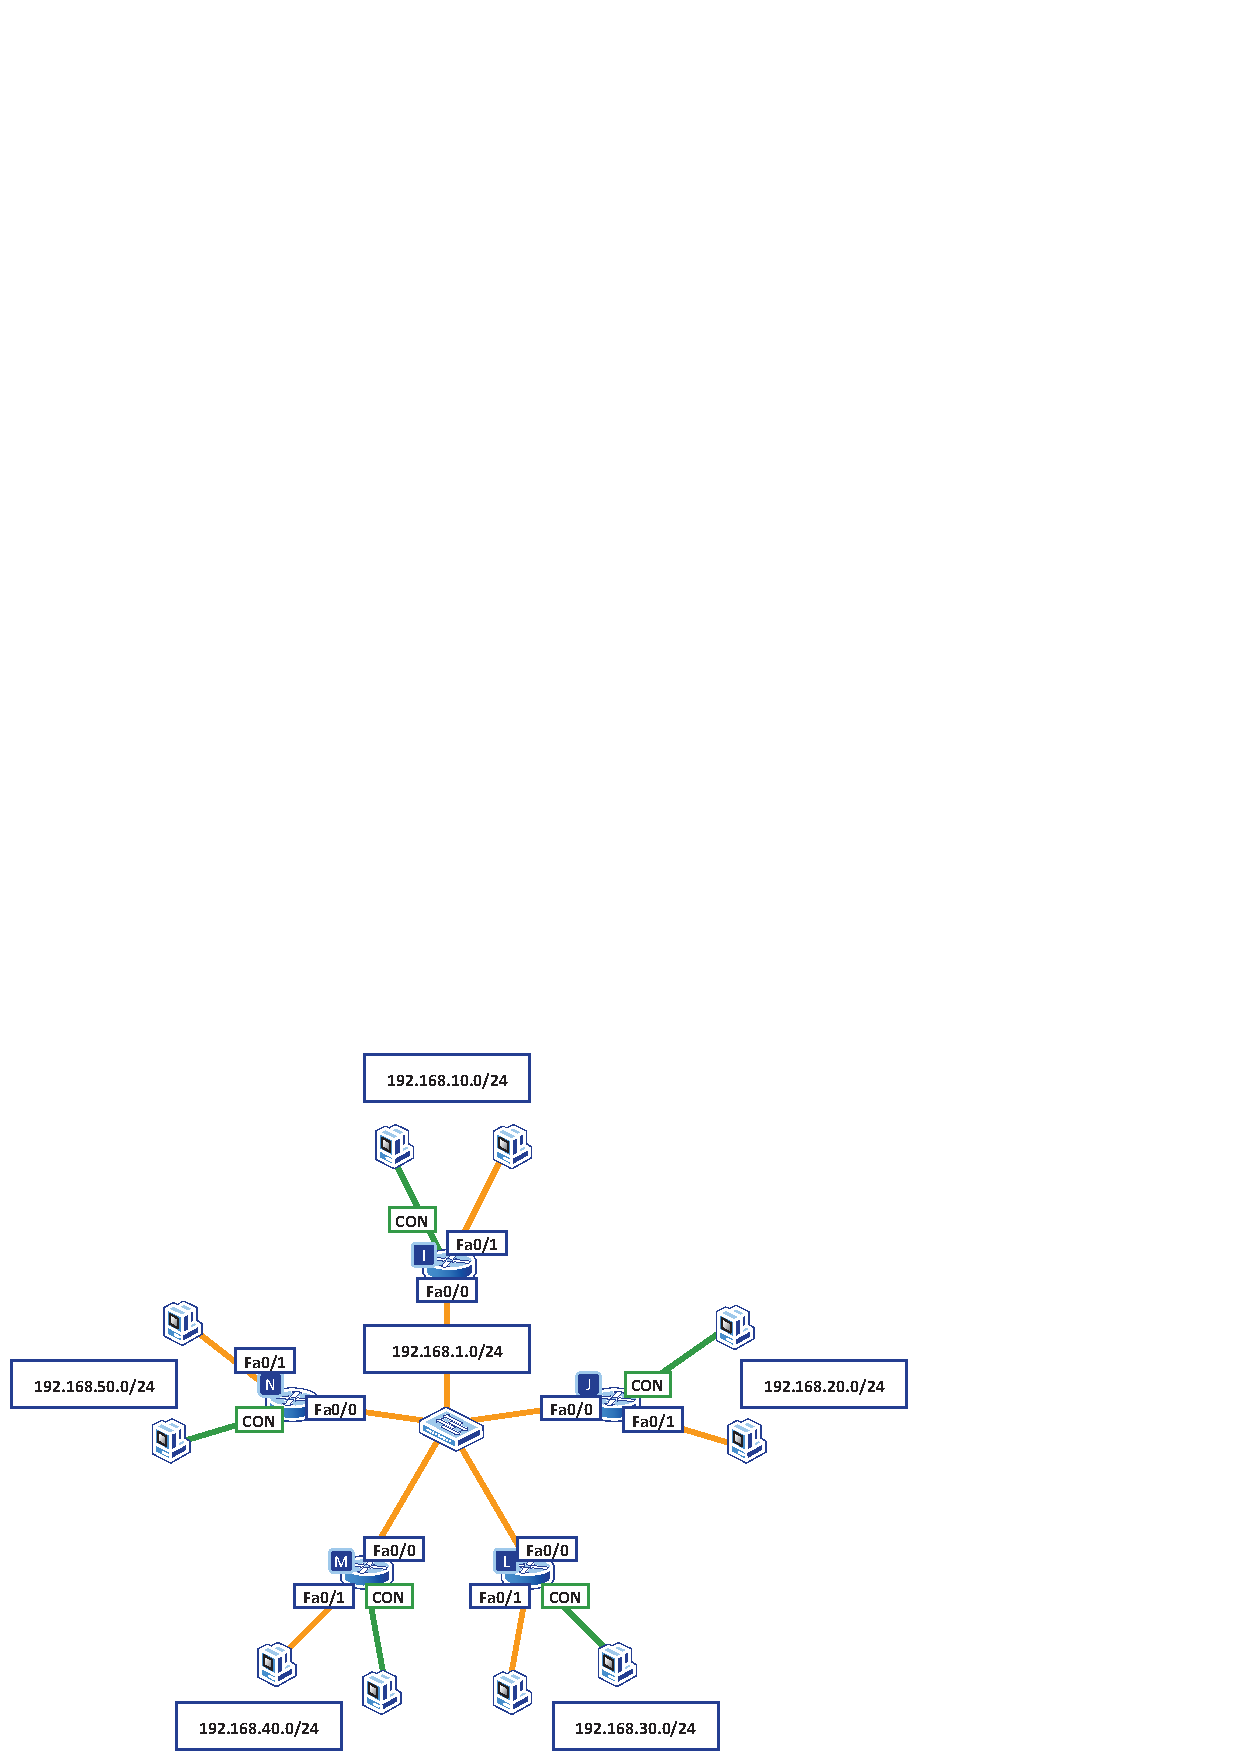
\includegraphics[width=0.9\linewidth]{Figures/RoutingEthernet.pdf}
\else
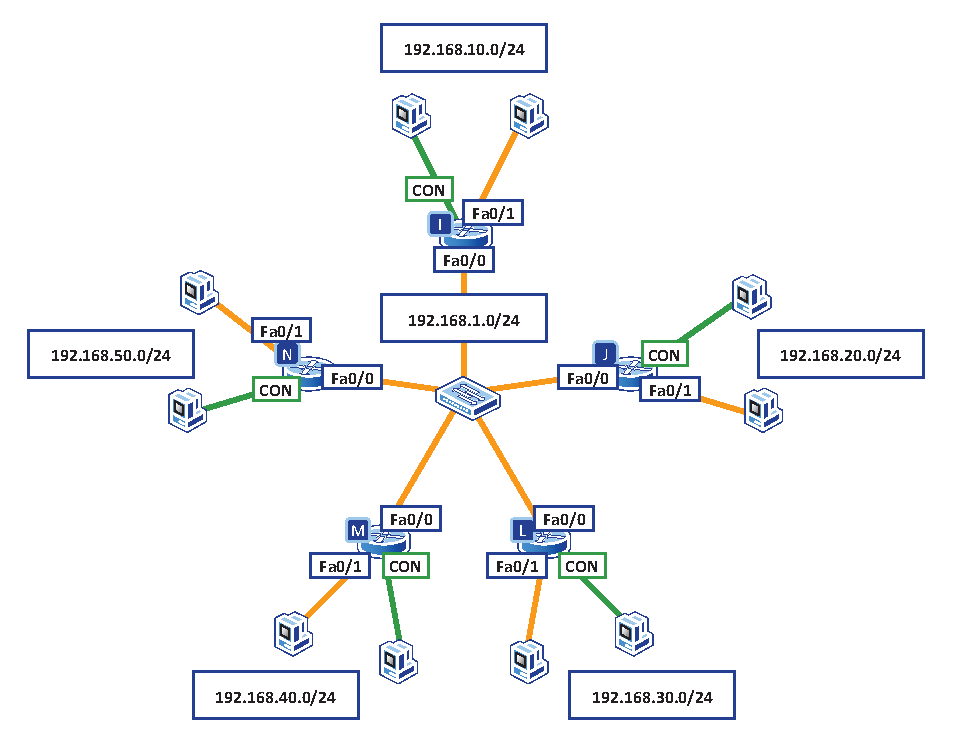
\includegraphics[width=0.9\linewidth]{Figures/RoutingEthernet.eps}
\fi
\caption{The network topology used for the Ethernet routing exercise.}
\label{fig:RoutingEthernet}
\end{figure}

The routers are connected to each other using the Ethernet interfaces and forming the topology from the figure \ref{fig:RoutingEthernet}. Use the console connection to connect to the routers (use \emph{PuTTY} to open a serial connection at 9600 bps). The COM port number (e.g. COM1, COM2, etc.) depends on your computer configuration\footnote{You can see the name of the local serial ports in the \emph{Device Manager} snap-in. To open the snap-in, click on \textsf{Start} \textgreater \textsf{Run...}, type \texttt{devmgmt.msc} and click \textsf{OK}. The serial ports are listed under the \emph{Ports} branch.}. The escape keystroke to exit the \texttt{ping} command in a router is \textsf{Ctrl-Alt-6}.

\subsection{Checking the Router Status}

Use the console to connect to your router and try the following commands. Prepare a summary of what you can see with each command.

\begin{lstlisting}
show history
show protocols
show interfaces
show ip route
\end{lstlisting}

\begin{center}
\sffamily\small
\begin{tabular}{>{\columncolor{tablegray}}p{15cm}}
\multicolumn{1}{>{\columncolor{tableorange}}l}{Questions \textbf{(4 $\times$ 3\,\%)}}\\
For each of the previous commands, what does the output represent?\\
\hline
\end{tabular}
\end{center}

\subsection{Create a Running and Startup Configuration}

Enter the privileged EXEC mode with the command:

\begin{lstlisting}
Router> enable
\end{lstlisting}

and password \texttt{\color{blue}cisco}, and the the global configuration mode

\begin{lstlisting}
Router# configure terminal
\end{lstlisting}

\begin{center}
\sffamily\small
\begin{tabular}{>{\columncolor{tablegray}}p{15cm}}
\multicolumn{1}{>{\columncolor{tableorange}}l}{Tasks \textbf{(4 $\times$ 3\,\%)}}\\
Find and include to your report the commands to:
\begin{itemize}
\item show and change the router name;
\item debugging mode configuration;
\item send pings from the router, and;
\item activate fair queueing on the ethernet interfaces (e.g. FastEthernet0/0).
\end{itemize}\\
\hline
\end{tabular}
\end{center}

Use the following commands to show and save the current configuration to the startup configuration from the privileged mode.

\begin{lstlisting}
Router# show running-config
Router# copy running-config startup-config
\end{lstlisting}

\subsection{IP Addresses Configuration}

Go to your physical router equipment and check which interfaces are visible. Use the following command to see what interfaces are available in the router.

\begin{lstlisting}
Router# show interfaces
\end{lstlisting}

\begin{center}
\sffamily\small
\begin{tabular}{>{\columncolor{tablegray}}p{15cm}}
\multicolumn{1}{>{\columncolor{tableorange}}l}{Tasks \textbf{(5\,\%)}}\\
Include in your report a table with the following information for each interface:
\begin{itemize}
\item the interface name;
\item the interface MTU;
\item the interface bandwidth, and;
\item the encapsulation protocol.
\end{itemize}\\
\hline
\end{tabular}
\end{center}

Enter in the configuration mode of the Ethernet interface with the command:

\begin{lstlisting}
Router(config)# interface <interface name>
\end{lstlisting}

Then, set the IP address to \texttt{192.168.{\color{red}X}0.1}, where \texttt{\color{red}X} is the number of your group. Use a /24 network mask. Use the IP address \texttt{192.168.{\color{red}X}0.2} for the Ethernet interface of your computer.

\begin{center}
\sffamily\small
\begin{tabular}{>{\columncolor{tablegray}}p{15cm}}
\multicolumn{1}{>{\columncolor{tableorange}}l}{Question \textbf{(5\,\%)}}\\
What is the command to configure the IP address on the router interface? Indicate the command mode in which you must execute this command.\\
\hline
\end{tabular}
\end{center}

Use the command:

\begin{lstlisting}
Router# show interfaces
\end{lstlisting}

to verify the IP address assignment, and enable the interface with the command:

\begin{lstlisting}
Router(config-if)# no shutdown
\end{lstlisting}

\begin{center}
\sffamily\small
\begin{tabular}{>{\columncolor{tablegray}}p{15cm}}
\multicolumn{1}{>{\columncolor{tableorange}}l}{Task \textbf{(5\,\%)}}\\
Include in your report the relevant output of at least one command showing that you successfully configured the IP address on the Ethernet interface.\\
\hline
\end{tabular}
\end{center}

Verify the line status and the interface status using the command:

\begin{lstlisting}
Router# show protocols
\end{lstlisting}

Use the commands:

\begin{lstlisting}
Router# show cdp neighbors
\end{lstlisting}

and:

\begin{lstlisting}
Router# show cdp neighbors detail
\end{lstlisting}

to see the neighboring Cisco devices.

\begin{center}
\sffamily\small
\begin{tabular}{>{\columncolor{tablegray}}p{15cm}}
\multicolumn{1}{>{\columncolor{tableorange}}l}{Question and Tasks \textbf{(5\,\%)}}\\
What are the devices displayed by the \texttt{show cdp neighbors} command? Write down the information received from the different interfaces.
\begin{itemize}
\item the neighbor identifier;
\item the IP address, and;
\item the port.
\end{itemize}\\
\hline
\end{tabular}
\end{center}

Use the \texttt{\color{blue}ping} command to test the connectivity to at least one other router in the lab.

\begin{center}
\sffamily\small
\begin{tabular}{>{\columncolor{tablegray}}p{15cm}}
\multicolumn{1}{>{\columncolor{tableorange}}l}{Task \textbf{(5\,\%)}}\\
Include in your report the output of the \texttt{\color{blue}ping} command, indicating the round-trip times.\\
\hline
\end{tabular}
\end{center}

From your computer, use the PuTTY in Telnet mode to connect to your router.

\begin{center}
\sffamily\small
\begin{tabular}{>{\columncolor{tablegray}}p{15cm}}
\multicolumn{1}{>{\columncolor{tableorange}}l}{Questions \textbf{(5 $\times$ 1\,\%)}}\\
Is it possible to remotely configure a router using Telnet?\\
\hline
Is login and password required?\\
\hline
Does a console user notice that there is an ongoing telnet connection?\\
\hline
Use telnet to change a parameter of the router (such as the router name) and verify the changes both using the console and the telnet connection. What happens?\\
\hline
Do any messages appear on the console when changes are done over Telnet? What information is included in these messages?\\
\hline
\end{tabular}
\end{center}

Logout the Telnet session to the Cisco router.

\subsection{IP Routing Configuration}

In this exercise, we shall enable the RIP protocol and check the status of the routing table as well as the RIP transactions of each router.

Check whether IP routing is enabled using the command:

\begin{lstlisting}
Router# show protocols
\end{lstlisting}

\begin{center}
\sffamily\small
\begin{tabular}{>{\columncolor{tablegray}}p{15cm}}
\multicolumn{1}{>{\columncolor{tableorange}}l}{Question \textbf{(5\,\%)}}\\
What is the status of IP routing?\\
\hline
\end{tabular}
\end{center}

Enter the global configuration mode and enter the submenu \texttt{\color{blue}router}.

\begin{center}
\sffamily\small
\begin{tabular}{>{\columncolor{tablegray}}p{15cm}}
\multicolumn{1}{>{\columncolor{tableorange}}l}{Question \textbf{(5\,\%)}}\\
What is the purpose of this submenu?\\
\hline
\end{tabular}
\end{center}

Use the \texttt{\color{blue}?} command to list available routing protocols and write down the results. Enter into the configuration of RIP.

\begin{lstlisting}
Router(config)# router rip
\end{lstlisting}

Use the command:

\begin{lstlisting}
Router(config-router)# network <network>
\end{lstlisting}

to associate your network to the RIP routing process. Assume that we are working with \emph{C} class IP addresses. Therefore, the last byte of the network address must be 0. Verify that the RIP protocol is now enabled and that your network has been recognized by the router using the command:

\begin{lstlisting}
Router# show ip protocol
\end{lstlisting}

\begin{center}
\sffamily\small
\begin{tabular}{>{\columncolor{tablegray}}p{15cm}}
\multicolumn{1}{>{\columncolor{tableorange}}l}{Task \textbf{(5\,\%)}}\\
Include in your report the output of the previous command showing that the RIP protocol has been enabled.\\
\hline
\end{tabular}
\end{center}

Observe the relevant parameters and answer the following questions:

\begin{center}
\sffamily\small
\begin{tabular}{>{\columncolor{tablegray}}p{15cm}}
\multicolumn{1}{>{\columncolor{tableorange}}l}{Questions \textbf{(3 $\times$ 2\,\%)}}\\
What timers do you identify for the RIP protocol?\\
\hline
What are their values?\\
\hline
What happens if we change the values?\\
\hline
\end{tabular}
\end{center}

Verify the status of the routing table with the command:

\begin{lstlisting}
Router# show ip route
\end{lstlisting}

\begin{center}
\sffamily\small
\begin{tabular}{>{\columncolor{tablegray}}p{15cm}}
\multicolumn{1}{>{\columncolor{tableorange}}l}{Task and Questions \textbf{(3 $\times$ 2\,\%)}}\\
Include in your report the routing table of your router, after the RIP protocol has been enabled on at least one other router in the lab.\\
\hline
What is the meaning of each of the fields in the table?\\
\hline
How do you identify the networks advertised using the RIP protocol?\\
\hline
\end{tabular}
\end{center}

\begin{center}
\sffamily\small
\begin{tabular}{>{\columncolor{tablegray}}p{15cm}}
\multicolumn{1}{>{\columncolor{tablered}}l}{Important}\\
For this assignment you must work together with another group. If there is no other group ready, skip this exercise and come back to it when another group reaches this point.\\
\hline
\end{tabular}
\end{center}

Add a static route to the other group's network. Use the following command from the configuration mode.

\begin{lstlisting}
Router(config)# ip route
\end{lstlisting}

\begin{center}
\sffamily\small
\begin{tabular}{>{\columncolor{tablegray}}p{15cm}}
\multicolumn{1}{>{\columncolor{tableorange}}l}{Task \textbf{(5\,\%)}}\\
Include in your report the command you used to setup a static route.\\
\hline
\end{tabular}
\end{center}

Use the \texttt{\color{blue}traceroute} command from your computer, choosing as destination the computer of another group.

\begin{center}
\sffamily\small
\begin{tabular}{>{\columncolor{tablegray}}p{15cm}}
\multicolumn{1}{>{\columncolor{tableorange}}l}{Question \textbf{(5\,\%)}}\\
Include the output of the traceroute command, indicating the network interfaces traversed by the traceroute ICMP or UDP packet?\\
\hline
\end{tabular}
\end{center}

Use the command:

\begin{lstlisting}
Router# debug ip rip
\end{lstlisting}

to show the RIP messages that are sent and received by the router.

\begin{center}
\sffamily\small
\begin{tabular}{>{\columncolor{tablegray}}p{15cm}}
\multicolumn{1}{>{\columncolor{tableorange}}l}{Questions \textbf{(2 $\times$ 2\,\%)}}\\
What are the source and destination of these packets?\\
\hline
What information do we obtain?\\
\hline
\end{tabular}
\end{center}

\subsection{Saving the Router Configuration in a TFTP Server}

A convenient way to store a router's configuration is using TFTP. We need to install the TFTP server in a computer with connectivity (layer 3 connectivity) to the router. Install the server and configure in which folder you want to save the router's configuration.

In the router, execute the command:

\begin{lstlisting}
Router# copy running-config tftp
\end{lstlisting}

and follow the instructions to enter the TFT server address (this is one of your computers) and the filename that you want to use. In the computer, open the configuration file using a text editor.

\begin{center}
\sffamily\small
\begin{tabular}{>{\columncolor{tablegray}}p{15cm}}
\multicolumn{1}{>{\columncolor{tableorange}}l}{Question \textbf{(5\,\%)}}\\
What is the format of the configuration file saved on your computer? How is the content of this file compared to the configuration file viewed in the router console?\\
\hline
\end{tabular}
\end{center}

To copy the configuration in the TFTP server to the router, there are two different options. Use either the command:

\begin{lstlisting}
Router# copy tftp running-config
\end{lstlisting}

on the server or simply copy and paste on the configuration terminal.

\section{Router Interconnection}

\begin{figure}
\centering
\ifpdf
\includegraphics[width=0.9\linewidth]{Figures/RoutingSerial.pdf}
\else
\includegraphics[width=0.9\linewidth]{Figures/RoutingSerial.eps}
\fi
\caption{The network topology used for the WAN routing exercise.}
\label{fig:RoutingSerial}
\end{figure}

In this session, we shall use the WAN (serial) interfaces of the routers. The figure \ref{fig:RoutingSerial} illustrates the topology of the network. In the previous session we used the Ethernet interfaces to connect the routers, and in this session we will use the serial interfaces.

\subsection{Shutdown the Ethernet Interfaces}

Make sure that there is no cable connected to the Ethernet interface, and that there is a cable connecting the serial interfaces. Delete the IP address of the Ethernet interface:

\begin{lstlisting}
Router(config-if)# no ip address
\end{lstlisting}

and administratively shutdown the interface:

\begin{lstlisting}
Router(config-if)# shutdown
\end{lstlisting}

Verify that the changes have been applied using:

\begin{lstlisting}
Router# show running-config
\end{lstlisting}

\begin{center}
\sffamily\small
\begin{tabular}{>{\columncolor{tablegray}}p{15cm}}
\multicolumn{1}{>{\columncolor{tableorange}}l}{Task \textbf{(5\,\%)}}\\
Include in your report the final configuration of the Ethernet interface.\\
\hline
\end{tabular}
\end{center}

\subsection{Configuration of the WAN Serial Interface}

The serial interfaces are interconnected by cables that, in the middle, have male/female connector. The router in the female connector side sets the communication rate. You can find which is the female router issuing the command:

\begin{lstlisting}
Router# show controller
\end{lstlisting}

The DTE interface uses the male connector, and the DCE interface uses the female connector. Alternatively, you may also look at the number on the cable, where 1428 is male and 1429 is female.

\begin{center}
\sffamily\small
\begin{tabular}{>{\columncolor{tablegray}}p{15cm}}
\multicolumn{1}{>{\columncolor{tableorange}}l}{Question? \textbf{(5\,\%)}}\\
What type of connector do you use for each of the serial interface?\\
\hline
\end{tabular}
\end{center}

From the privileged mode of your router, enter the global configuration mode. Enter into the configuration of the WAN serial interface and configure the IP.

To choose the IP, use the following algorithm. Assume the your group id is \texttt{\color{red}X} and your neighbor's group ID is \texttt{\color{red}Y}. If \texttt{\color{red}X} \textless \texttt{\color{red}Y}, then your IP is \texttt{192.168.{\color{red}XY}.1}. Otherwise, it is \texttt{192.168.{\color{red}YX}.2}. Use a /30 network mask.

\begin{center}
\sffamily\small
\begin{tabular}{>{\columncolor{tablegray}}p{15cm}}
\multicolumn{1}{>{\columncolor{tableorange}}l}{Task \textbf{(5\,\%)}}\\
Include in your report the commands you used to setup the IP addresses on each serial interface.\\
\hline
\end{tabular}
\end{center}

On the DCE serial interface, you must setup the interface clock rate. Using this practical exercise we shall use a clock rate of 128 kbps. Use the command:

\begin{lstlisting}
Router(config-if)# clock rate <bps>
\end{lstlisting}

or the closest available rate.

Verify the previous configuration is correct and enable the serial interfaces using the command:

\begin{lstlisting}
Router(config-if)# no shutdown
\end{lstlisting}

\begin{center}
\sffamily\small
\begin{tabular}{>{\columncolor{tablegray}}p{15cm}}
\multicolumn{1}{>{\columncolor{tableorange}}l}{Task \textbf{(10\,\%)}}\\
Include in your report the final configuration of the serial interfaces.\\
\hline
\end{tabular}
\end{center}

Wait for your neighbors to complete their configuration, and then use the command:

\begin{lstlisting}
Router# show protocols
\end{lstlisting}

to verify the state of the line.

\begin{center}
\sffamily\small
\begin{tabular}{>{\columncolor{tablegray}}p{15cm}}
\multicolumn{1}{>{\columncolor{tableorange}}l}{Task \textbf{(5\,\%)}}\\
Include in your report the state of each serial interface.\\
\hline
\end{tabular}
\end{center}

Now we will gather information about neighboring devices using the command:

\begin{lstlisting}
Router# show cdp neighbors
\end{lstlisting}

or

\begin{lstlisting}
Router# show cdp neighbors detail
\end{lstlisting}

\begin{center}
\sffamily\small
\begin{tabular}{>{\columncolor{tablegray}}p{15cm}}
\multicolumn{1}{>{\columncolor{tableorange}}l}{Task \textbf{(10\,\%)}}\\
Elaborate a table indicating, for each neighbor, the following information:
\begin{itemize}
\item the neighbor identifier;
\item the neighbor IP address, and;
\item the port.
\end{itemize}\\
\hline
\end{tabular}
\end{center}

Enable routing using the following commands:

\begin{lstlisting}
Router(config)# ip routing
Router(config)# router rip
Router(config-router)# network <network>
\end{lstlisting}

and look at the routing tables using the command

\begin{lstlisting}
Router# show ip route
\end{lstlisting}

\begin{center}
\sffamily\small
\begin{tabular}{>{\columncolor{tablegray}}p{15cm}}
\multicolumn{1}{>{\columncolor{tableorange}}l}{Tasks \textbf{(2 $\times$ 5\,\%)}}\\
Include in your report the current routing table.\\
\hline
Compare the routing table to the one obtained in the previous session and highlight the differences.\\
\hline
\end{tabular}
\end{center}

Use the \texttt{\color{blue}ping} tool to measure the connectivity to the other routers in the network.

\begin{center}
\sffamily\small
\begin{tabular}{>{\columncolor{tablegray}}p{15cm}}
\multicolumn{1}{>{\columncolor{tableorange}}l}{Tasks \textbf{(2 $\times$ 5\,\%)}}\\
Indicate which routers are reachable and which are not. Explain why by using the current routing table.\\
\hline
Are there differences in the round-trip-time compared to the measures taken in the previous session? Why?\\
\hline
\end{tabular}
\end{center}

\subsection{Network Topology}

{\color{red}\textbf{(30\,\%)}}

Compare the current network topology to one of the previous session. Answer in a few brief sentences to the following questions.

\begin{center}
\sffamily\small
\begin{tabular}{>{\columncolor{tablegray}}p{15cm}}
\multicolumn{1}{>{\columncolor{tableorange}}l}{Questions \textbf{(3 $\times$ 10\,\%)}}\\
What are the differences between the two networks? Enumerate at least three (3).\\
\hline
What are the advantages of the current topology over the previous one?\\
\hline
What are the disadvantages of the current topology over the previous one?\\
\hline
\end{tabular}
\end{center}

\section{Configuration of an L2-L3 Network}

\begin{figure}
\centering
\ifpdf
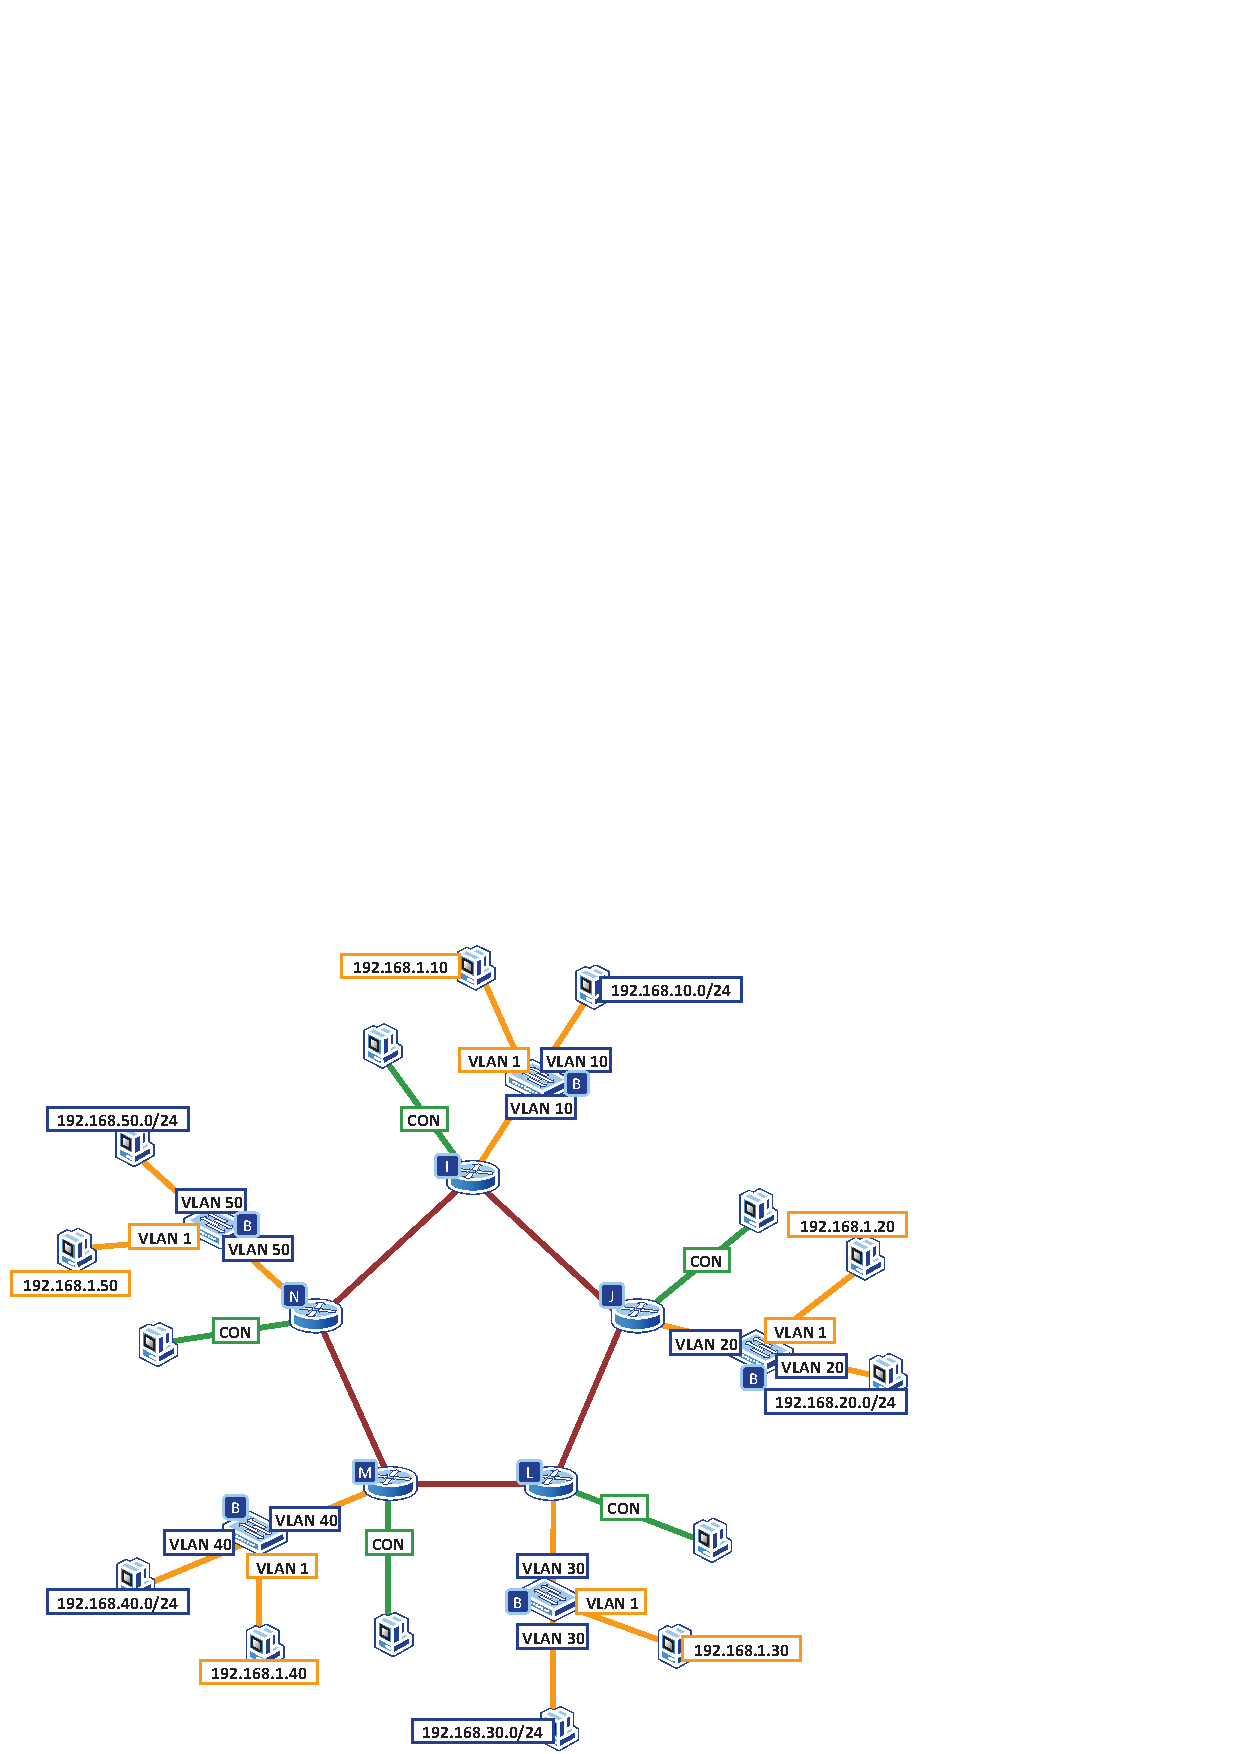
\includegraphics[width=0.9\linewidth]{Figures/RoutingSwitches.pdf}
\else
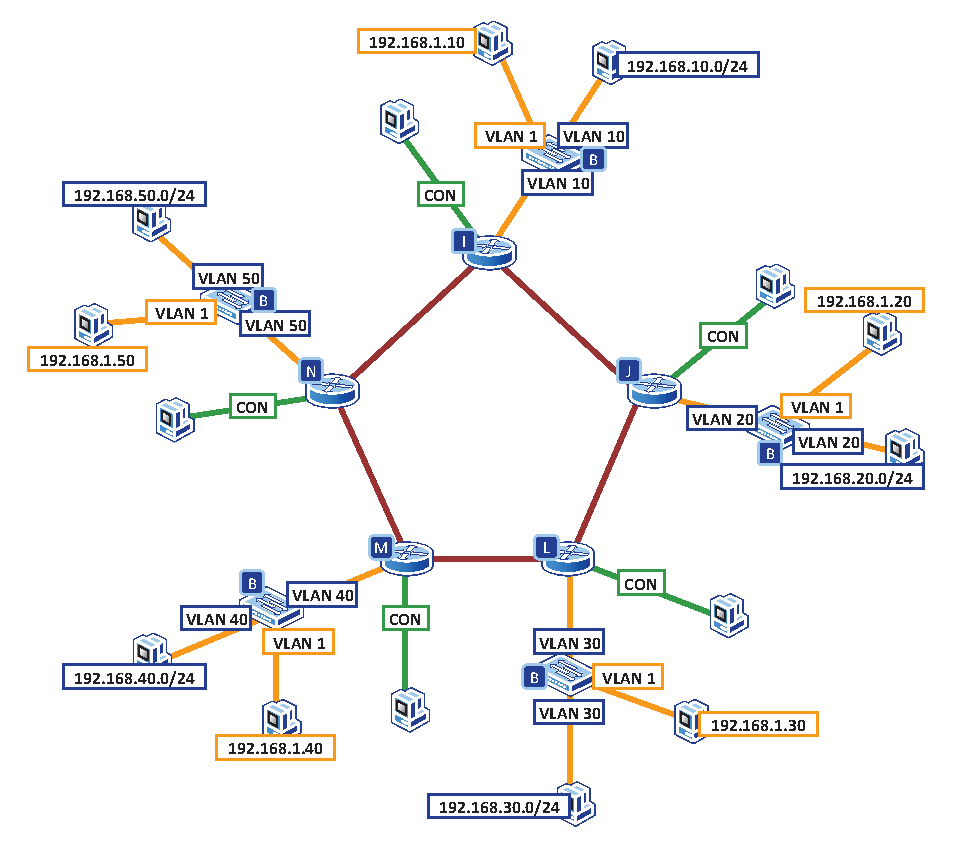
\includegraphics[width=0.9\linewidth]{Figures/RoutingSwitches.eps}
\fi
\caption{The network topology used for the L2-L3 network.}
\label{fig:RoutingSwitches}
\end{figure}

This third session extends the previous one by including switches to the network topology, as shown in the figure~\ref{fig:RoutingSwitches}. The topology consists of a ring of routers connected in a ring using the serial interfaces. Each router is connected using the Ethernet interface to a local area network with two or more computers. The devices used in this assignment are:

\begin{itemize}
\item computers;
\item up to six Cisco routers with an ethernet interface and two serial interfaces;
\item up to three Cisco switches, and;
\item direct and cross-over RJ-45 cables.
\end{itemize}

Each group has to configure its router and its VLAN. It is assumed that the previous session has been successfully completed and the connectivity tests were satisfactory.

\subsection{VLAN Configuration}

{\color{red}\textbf{(40\,\%)}}

We connect using Telnet to our switch and enter the privileged EXEC mode. Create a VLAN with a number equal to ten times your group number (e.g. VLAN 20 for group 2). Assign a port connected to the router and one or two other ports connected to computers. Remember to keep the port of the computer you are using for managing the switch in VLAN 1.

Use an IP equal to 192.168.1.XX where XX is the group multiplied by ten for the computer in VLAN 1. Use an IP 192.168.VLAN.YY for the other VLAN. YY is going to be 1 for the router and 2 for the computer. You can use YY equal to 3 if you have another computer.

Test the connectivity between your different computers and with computers of other groups. Write down when a \texttt{\color{blue}ping} command is successful and when it is not successful, and provide an explanation.

\subsection{Configuring the Router LAN Interface}

{\color{red}\textbf{(40\,\%)}}

In the router console enter the privileged EXEC mode and use the command:

\begin{lstlisting}
Router# show interfaces
\end{lstlisting}

to see the interfaces which are available in the router. We enter the global configuration mode and in in the configuration of the LAN (Ethernet) interface. We configure the IP for this interface. Then we enable the interface with the command:

\begin{lstlisting}
Router(config-if)# no shutdown
\end{lstlisting}

and check the link status LED. We can also check the status of the line and the interface using the command:

\begin{lstlisting}
Router# show protocols
\end{lstlisting}

Then we enable the routing. From the global configuration menu we enter the router menu and we use the command:

\begin{lstlisting}
Router(config-router)# network 192.168.VLAN.0
\end{lstlisting}

to associate our network to the routing process. We will assume that we are using class C networks. Then we use the command:

\begin{lstlisting}
Router# show routes
\end{lstlisting}

to see the routing tables.

\subsection{Connectivity Test}

{\color{red}\textbf{(20\,\%)}}

We add our router's IP as as the default gateway for the computers connected to the router. We perform ping tests from the router to the other devices of the network. Finally, we fill in a table with the following information:

\begin{itemize}
\item the destination IP address;
\item the packet loss, and;
\item the average delay.
\end{itemize}

Now we repeat the tests from the computer. If we are on a Linux box, we may also try the \texttt{\color{blue}tracepath} and \texttt{\color{blue}mtr} commands. We will include the configuration of the switch and the router in the lab assignment report.

